\chapter{Semantic Connection}

\section{Advantages of semantic information}

\begin{figure}[h]
\centering
%self
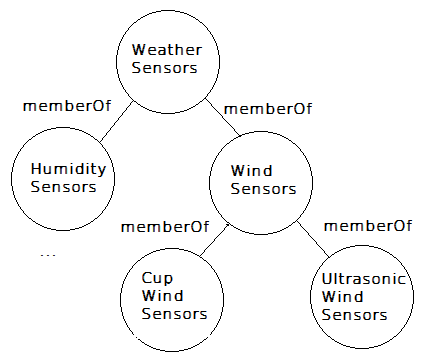
\includegraphics[width=0.6\textwidth]{figures/semws.png}
\caption{Using triples in the example\label{fig:semws}}
\end{figure}

In a cyberphisical system stored in an SOS every sensor has a name and a type. These are identifiers that correspond to a sensor and there may be other descriptors that are not informative for human reader. Sensors can be called on different names like Anemometer, Wind instrument, wind meter that means the same, measures the speed of the wind. Filtering for name is not a good approach for filtering the information. To make monitoring simpler. A semantic information is needed that organizes the data in a way that is convenient for the human reader to read. The sensors should be separated into different groups and subgroups and these groups should have an easily distinguishable name. Such groups can be Phyisical sensors -> Weather Sensors -> Wind sensors -> Wind speed sensors. This information yet can not be stored on the SOS server a separate ontology database shall be created. 
The usual way to store such information is in an ontology. 
An ontology is a description where objects, their properties and the connections between objects are described. This is very similar to classes, instances and relations in object oriented programming. An example of Java classes translated to an RDF ontology can be seen on Figure \ref{fig:rdf}\cite{g2d4}.


\begin{figure}
        \centering
        \begin{minipage}[b]{0.4\textwidth}
\begin{verbatim}

// classes
class Style {
 String neve;
}
class MusicalStyle 
	extends Style {
}
class Author {
 MusicalType musicalType;
}
// instances
MusicalType classic
 = new MusicalType();
Author Mozart =
 new Author();
Mozart.style = classic;
\end{verbatim}

        \end{minipage}
        \begin{minipage}[b]{0.4\textwidth}
        \begin{verbatim}

<!-- classes -->
<rdfs:Class rdf:id="Style"/>
<rdfs:Class rdf:id="MusicalStyle">
 <rdfs:subClassOf rdf:resource="#Style"/>
</rdfs:Class>
<rdfs:Class rdf:id="Author"/>
<!-- attributes -->
<rdf:Property rdf:id="StyleName">
 <rdfs:domain rdf:resource="#Style"/>
 <rdfs:range STRING/>
</rdf:Property>
<rdf:Property rdf:id="musicalStyle">
 <rdfs:domain rdf:resource="#Author"/>
 <rdfs:range rdf:resource="#MusicalStyle"/>
</rdf:Property>
<!-- instances -->
<MusicalStyle rdf:id="classic"/>
<Author rdf:id="Mozart">
 <MusicalStyle rdf:resource="#classic"/>
</Author>               
\end{verbatim}

        \end{minipage} 
 \caption{Java classes and their RDF representation side by side}
                \label{fig:rdf}
\end{figure}
The most widespread ontology storage standards are the RDF databases.

\section{Resource Definition Framework}

The RDF standard\cite{rdf} is created to be used with the Semantic Web approach to expand web pages with additional meanings that makes machines capable of understanding and reasoning about a web page. For example a web store can be easily understand by a customer: it has items, prices, shipping information, etc. However, for machines without saying explicitly that the value in one field is the price in USD it can be easily confused by the dimensions or the performance. Although nowadays these problems can be solved by machine learning, it is still a resource intensive process. To solve this problem an XML based standard has been introduced. This is done by using triples. 

The triple describes \textit{which} page or entity (subject) is connected on \textit{what} property(predicate) to \textit{which} other page or entity(object). These triples are separate three unique values and it is called a statement.
Each value could have another triple describing it. The first (subject) part is the resource  which we make statements from. The second parameter (predicate) is the property of the resource that represents the attribute, aspect or connection. The third parameter is the value(object) which can refer to other resources or it can be a value from a specific domain like a number. This is very similar to statements in real life, like:
\begin{itemize}
\item Anemometer measures wind-speed
\item Anemometer is a wind-sensor
\item Wind-sensor is a sensor
\end{itemize} 
From the above example direct connections between wind-sensors and Anemometer can be described. Using reasoning indirect connections can be deduced. This makes RDF databases a powerful schema to describe real world examples. To be able to describe a big ontology which were put together using multiple ontologies each unique resource identifier is a fully qualified domain name and a hash tag and a unique name, like a URL with an anchor on a web page. 
The original idea behind the fully qualified domain name is that the approach was designed to give semantic meanings for web pages. 
Pages could refer to each other and give a global knowledge that is understandable by computers too. 

Such recursive data can be represented in graph databases, where reasoning is only walking in the database. There are graph databases to store these triples and also dedicated RDF databases. The standard way to query RDF databases is using SPARQL queries. Although RDF can represent data and connections it can not describe the rules how the reasoning, the walks in the graph should be done. These are represented by OWL or SWRL which are an extension to the RDF. However, most RDF databases also support such rules.

Raw RDF descriptor files are stored in XML format. A comparison beween classes and their RDF representation can be seen on \ref{fig:rdf}.


\begin{figure}[h]
\centering
%http://blog.52north.org/2014/02/21/sos-js/
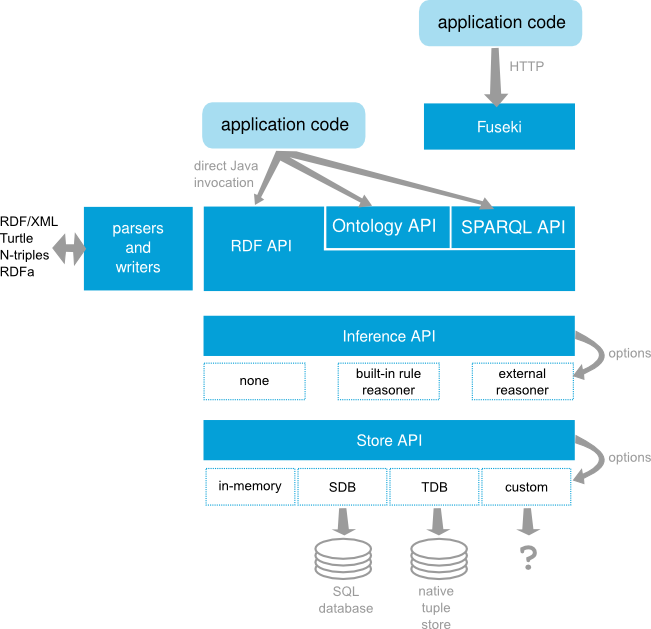
\includegraphics[width=0.6\textwidth]{figures/jena-architecture.png}
\caption{Architecture of Apache Jena\label{fig:jena}}
\end{figure}


\section{Some open source RDF databases} 

Apache Jena is an open source RDF datastore supported by the Apache foundation. It is written in Java\cite{jena}. It has many interfaces and supports many database backends. It can be used with in memory databases, SQL RDBs, triplestores. There is a built-in reasoner in the datastore, however it can be changed to other external reasoners too. The architecture of the software is shown on Figure \ref{fig:jena}.

OpenRDF Sesame is another tool for storing RDF triples. It is also written in Java. It has three different interfaces for communication: the SAIL API, the RIO interface and an HTTP client. The whole application runs from a Java container like Tomcat.

Apache Foundation also supports another RDF and Graph related project called Apache Marmotta. It was started in 2012. It supports a wide range of datastore engines from in memory databases through SQL servers to large distributed column bases stores like Apache Cassandra. 

There is an out of the box tool that contains better reasoners, has a basic GUI and accepts different data types. This is Stardog database. It is a commercial application. However, it has a community version with a few restrictions. The software is written in Java and run from a web container, like Tomcat. It supports many interfaces such as HTTP and SNARL, it has a built in reasoner with integrated constraint validation. Connectors for different programming languages are ready to use. It can be easily queried using SPARQL. It has support for OWL 2 rules. Because it is an easy to use, out of the box tool this database  is used in the sample application.

\begin{figure}[h]
\centering
%http://openrdf.callimachus.net/sesame/2.7/docs/articles/figures/sesame-components.png
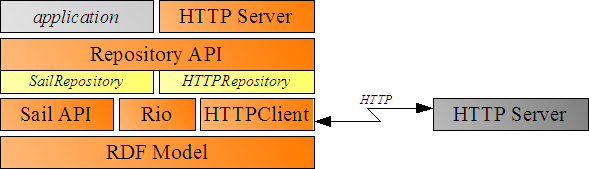
\includegraphics[width=0.6\textwidth]{figures/sesame-components.png}
\caption{Components of Sesame\label{fig:sesame}}
\end{figure}

\section{SPARQL for the queries}

To retrieve the necessary metadata the SPARQL query language is used in the RDF databases. These queries are less human readable than standard SQL queries, although they look similar. The language builds on the subject-predicate-object triples. In a result all matching data is responded. 

\begin{lstlisting}[caption={Sample SPARQL that queries all filterable objects\label{lst:sparql}}]
select ?s { <uri#filterable> <uri#subPropertyOf> ?s }
\end{lstlisting}

A SPARQL query can be quite complex. A simple query can be seen on listing \ref{lst:sparql}. A query can start with a BASE attribute, which defines the default prefix for each attribute. When this base is defined, it can be neglected from the query itself. As these are usually long URL-s, this can have a big gain on query length. The second given attributes are the prefixes. If external nodes from external sources are referenced, it can be shortened by using a prefix. This also results a shorter query. The next given parameter can be after a SELECT keyword a list separated by commas of the fields that should be displayed in the output. These are the variables that have been used in the condition. 
The condition part starts with the WHERE keyword. After that comes a multiple list of triples, where one keyword is either displayed in the result or have a reference in the query chain. If two triple can be either connected with a comma, a semi-colon or a dot. If it is a dot it means that the statement is finished the subject, predicate, object values are given. Having a semi-colon as a separator means that the subject should be repeated, only the predicate and the object is needed. The comma repeats the subject and the predicate, this way only the other object is needed. The prefix is separated by a colon from these values. Filtering functions can be also given in a query. For example the FILTER function can have one parameter and a regular expression and it filters only those values which fulfill the given regular expression. It can also compare values. Results can be grouped, ordered, just like in standard SQL languages. Aggregation of results are also possible. 

A SPARQL query can also provide other answers than returning a list of the answers. SELECT can be replaced by CONSTRUCT for creating new triples or by ASK which will check if the value exists in the repository. 


\begin{lstlisting}[caption={Sample complex SPARQL which shows top 5 countries based on population using DBpedia\label{lst:sparqlcomplex}}]
PREFIX type: <http://dbpedia.org/class/yago/>
PREFIX prop: <http://dbpedia.org/property/>
SELECT ?country_name ?population
WHERE {
?country a type:LandlockedCountries ;
rdfs:label ?country_name ;
prop:populationEstimate ?population .
FILTER (?population > 15000000 && langMatches(lang(?country_name), "en")) .
} ORDER BY DESC(?population) LIMIT 5
\end{lstlisting}

With such technology the triples can be stored and retrieved. However, the ontology behind the measurement is still missing. For that there is a standard ontology for sensors maintained by the Semantic Sensor Network Incubator Group. The underlying system which will be introduced in the next chapter is using this ontology in a somewhat customized way\cite{g2d2}.  The ontology is described in the next section.

\section{The Semantic Sensor Network Ontology}

The Semantic Sensor Network Incubator Group is a W3C incubator project. These projects are ran for one year to work on an area, this project ran from March of 2009 to September of 2010. It has developed an ontology for the semantic annotation of the Sensor Web Enablement standard. The ontology is available at http://www.w3.org/2005/Incubator/ssn/ssnx/ssn website, and it is conceptually organized into 10 modules. This is only a conceptual representation, the implementation consists of 41 concepts and 39 object properties. Part of its objects can be seen on Figure \ref{fig:ssnopart}.It is built upon a lightweight ontology, the  DOLCE-UltraLite. This underlying ontology helps the new one to connect with other semantic databases and to have a better understanding of the concepts behind the properties. 


\begin{figure}[h]
\centering
%custom
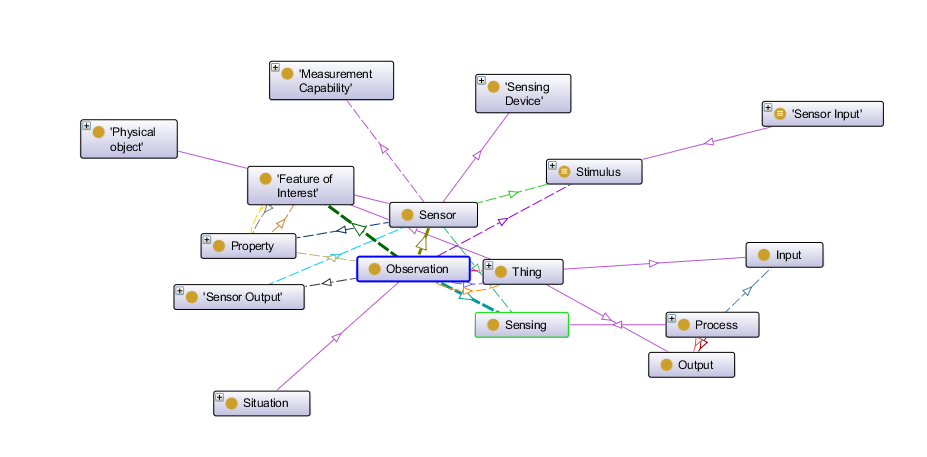
\includegraphics[width=0.6\textwidth]{figures/ssnopart.png}
\caption{Parts of the SSN Ontology\label{fig:ssnopart}}
\end{figure}

The ontology can be viewed from four different perspectives:
\begin{itemize}
\item A sensor perspective with focus on what and how it senses and what it sensed.
\item An observation perspective which focuses on the observation and its environment.
\item A system perspective in focus on the network itself and the deployment.
\item A feature and property perspective which focuses on the physical properties and the subject of the observation. 
\end{itemize}
This makes it possible not just to deduct that for example wind sensor is a kind of sensor but that wind speed is a speed measurement. The connections between each object of the SSN ontology using reasoning can be seen on Figure \ref{fig:ssninfer}. 
In every ontology the ancestor is the Thing object. Its descendants are the Entities and the Input and Output objects. An entity can be an Event, like a measurement (sensor input), a process or an action. A sensor input is triggered by a Stimulus (stimulation of the sensor). The properties of the sensors are also Entities. There are two kind of properties, one is the property of the measurement and the other is the property of the sensor itself.

\begin{figure}[h]
	\centering
	%custom
	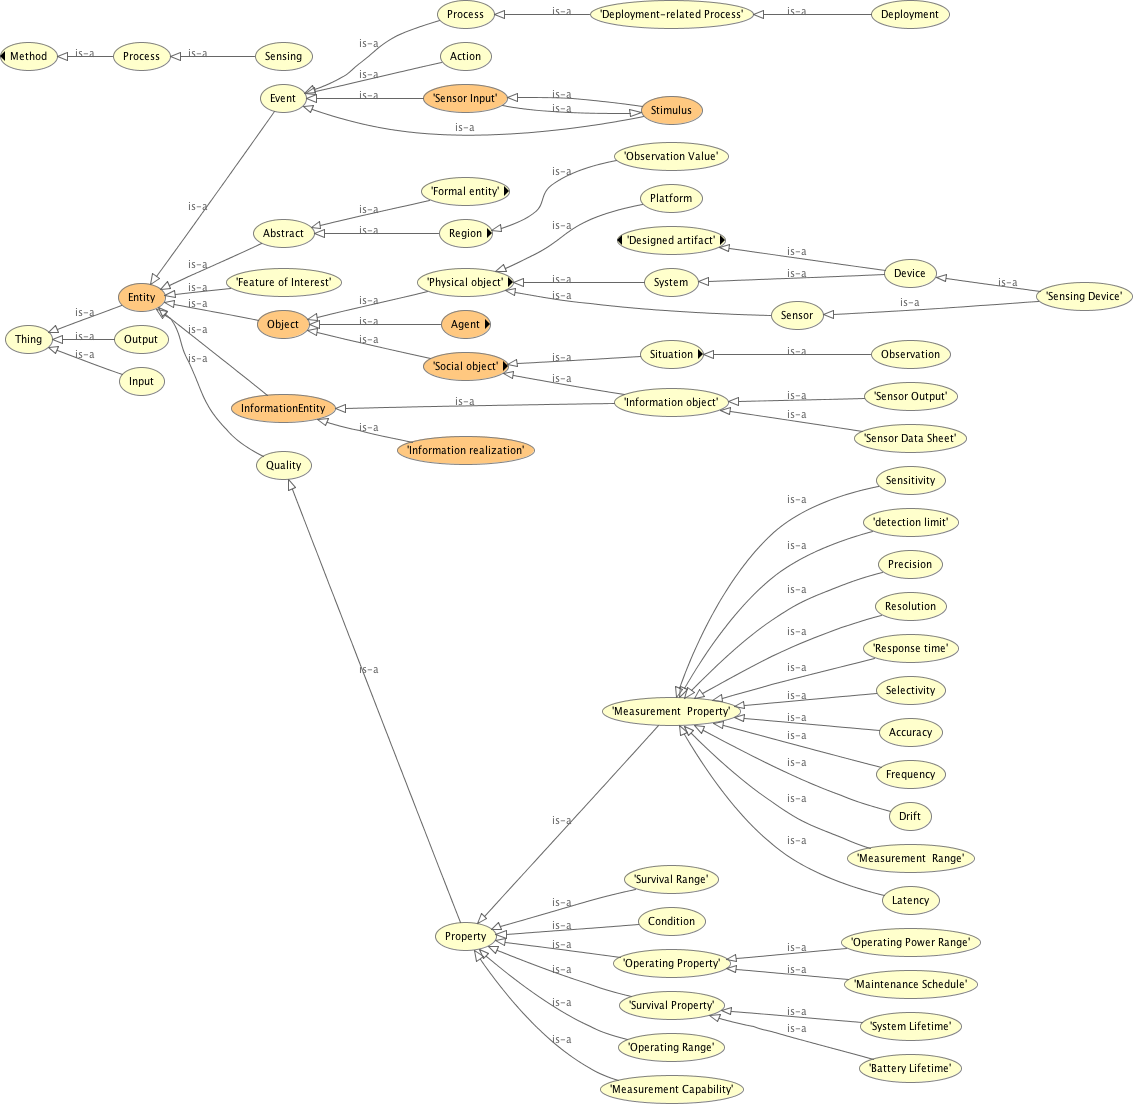
\includegraphics[width=0.9\textwidth]{figures/ssno-infer.png}
	\caption{Inferenced connections of the SSNO\label{fig:ssninfer}}
\end{figure}
